\documentclass[12pt,oneside,slovak,a4paper]{article}

\usepackage[slovak]{babel}
\usepackage[utf8]{inputenc}
\usepackage{amsmath}
\usepackage{amsfonts}
\usepackage{amssymb}
\usepackage{graphicx}
\usepackage{cite}
\usepackage[IL2]{fontenc} % lepšia sadzba písmena Ľ než v T1
\usepackage{pdfpages}
\usepackage[hyphens]{url} % príkaz \url na formátovanie URL, [hyphens] fixne formatovanie v literature
\usepackage[hidelinks]{hyperref} % odkazy v texte budú aktívne (pri niektorých triedach dokumentov spôsobuje posun textu)
\usepackage[left=2cm,right=2cm,top=2cm,bottom=2cm]{geometry}
\usepackage{float}
\usepackage[normalem]{ulem}
\useunder{\uline}{\ul}{}
\usepackage{titling}
\usepackage{xcolor}
\usepackage{lipsum}
\usepackage{setspace}
\usepackage{blindtext}
\usepackage{caption}
\usepackage{tabularx}
\usepackage[numbers]{natbib}
\usepackage{color}




% riadkovanie 1.5
\begin{document}
\linespread{1.5}\selectfont

\begin{titlepage}
	\centering
    {\Large Slovenská technická univerzita v Bratislave\par}
    {\Large Fakulta informatiky a informačných technológií\par}
	\vspace{7cm}
	{\huge\bfseries Spoľahlivý systém ukladania osobných dát v domácnosti\par}
	\vspace{0.5cm}
    {\Large \textsc{Projektovanie aplikácií počítačov}\par}
    \vspace{1cm}
	{\Large\itshape Marek Čederle\par}
    {\small\texttt{xcederlem@stuba.sk}\par}
	\vfill

	{\large \today\par}
\end{titlepage}


% ----------------- Obsah -----------------
\tableofcontents
\vspace*{\fill}
\newpage

% ----------------- Kapitoly -----------------

% vsetky zdroje z literatura.bib aby sa zobrazili bez citovania
\nocite{*}

\section{Úvod}
V dobe, kedy digitálne údaje sú veľmi dôležité nielen pre firmy, ale aj pre jednotlivcov, je nevyhnutné mať spoľahlivé riešenie na ukladanie a zálohovanie údajov. Tento projekt sa zameriava na implementáciu spoľahlivého systému ukladania a zálohovania údajov, ktorý môže bežná osoba prevádzkovať v pohodlí svojho domova. Pôjde o vytvorenie systému NAS\footnote{Network Attached Storage} využívajúcej bežne dostupné počítačové komponenty a sieťovú infraštruktúru. Projekt sa venuje aj výberu vhodného softvéru, ktorý efektívne využije možnosti systému NAS. Okrem toho sa zaoberá umiestnením NAS v domácom prostredí, aby bolo zabezpečené pohodlné používanie bez zbytočného rušenia. Dôležitou súčasťou projektu je aj porovnanie nákladov medzi domácou a komerčnou alternatívou.

\section{Hardvér}
Pre potreby projektu som sa snažil vyberať hardvér ktorý má najvyšší pomer cena/výkon. Taktiež som sa snažil vyberať komponenty ktoré sú dostupné na slovenskom trhu. Po výbere a predstavení komponentov si náš systém následne poskladáme.

\subsection{PC Skriňa}
Pre naše potreby nám bude stačiť PC skriňa Franctal Design CORE 2500, ktorá je dostatočne veľká na to aby sme do nej mohli nainštalovať všetky potrebné komponenty. Obsahuje aj dostatok pozící pre dátové disky ktorých sa do 3,5'' slotov zmestí až 4 a následne pomocou redukcie do 5,25'' až 2 čo nám dohromady dáva priestor pre 6 diskov.

% obrazok PC skrine
\begin{figure}[H]
	\centering
	\captionsetup{justification=centering,margin=2cm}
	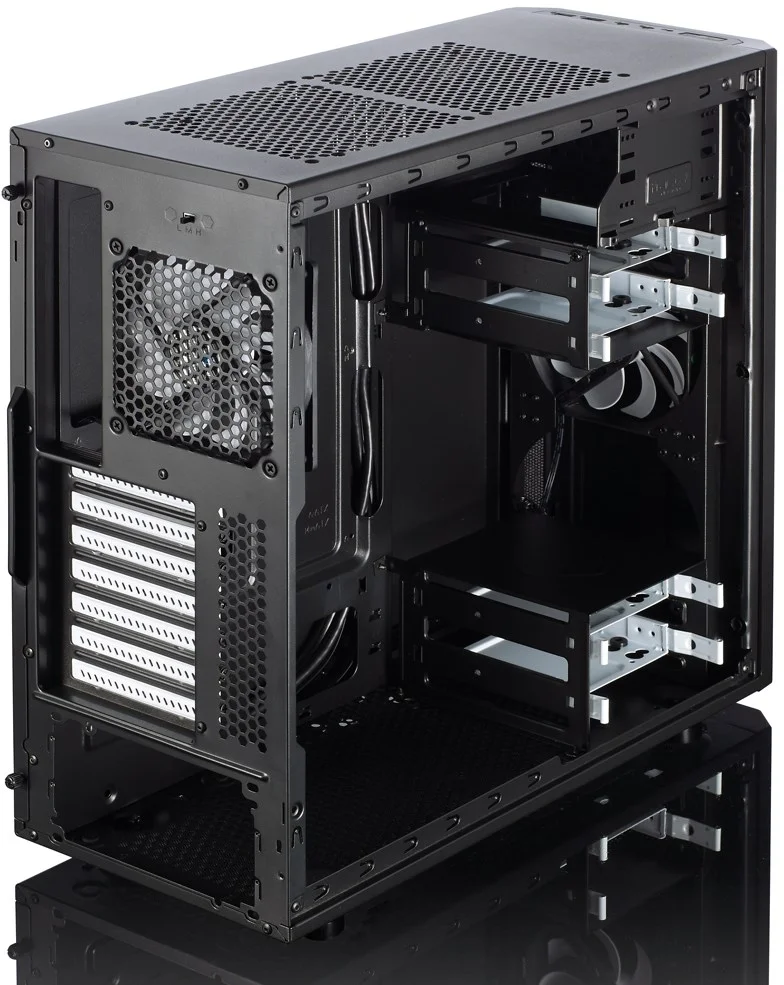
\includegraphics[width=\linewidth]{./images/case.png} % mozno pouzit scale=0.5
	\centering
	\caption{PC Skriňa - Fractal Design CORE 2500 \\ Zdroj: https://www.alza.sk/fractal-design-core-2500-d2169926.htm}
\end{figure}

%tabulka špecifikacii skrine
\begin{table}[h]
\centering
\begin{tabular}{|l|l|}
\hline
\textbf{Parameter} & \textbf{Hodnota} \\ \hline
Veľkosť & Midi Tower \\ \hline
Farba & Čierna \\ \hline
Formát základnej dosky & ATX, mATX (Micro ATX), mITX (Mini ITX) \\ \hline
Počet interných 3,5" slotov & 4× \\ \hline
Počet interných 2,5" slotov & 1× \\ \hline
Max. výška chladiča procesora & 162 mm \\ \hline
Max. dĺžka grafickej karty & 380 mm \\ \hline
Ďalšie vybavenie & Prachové filtre \\ \hline
Externá 5,25" pozícia & 2× \\ \hline
Umiestnenie predného panelu & Zhora \\ \hline
Konektory predného panelu & USB 3.2 Gen 1, Slúchadlá, Mikrofón \\ \hline
Bočnica & Nepriehľadná \\ \hline
Materiál bočnice & Oceľová \\ \hline
Regulácia ventilátorov & Áno \\ \hline
Zdroj & Bez zdroja \\ \hline
Podporovaný formát zdroja & ATX \\ \hline
Veľkosť predného ventilátora & 1x120mm, 2x140mm \\ \hline
Veľkosť zadného ventilátora & 1x120mm \\ \hline
Veľkosť horného ventilátora & 1x120mm, 1x140mm \\ \hline
Počet pozícií pre ventilátory & 7× \\ \hline
Počet osadených ventilátorov & 2x120mm \\ \hline
Podporovaná veľkosť radiátora zhora & 120mm, 240mm \\ \hline
Podporovaná veľkosť radiátora spredu & 120mm, 140mm, 240mm, 280mm \\ \hline
Farba podsvietenia & Bez podsvietenia \\ \hline
Materiál skrine & Oceľ \\ \hline
Šírka & 195 mm (19,5 cm) \\ \hline
Výška & 431 mm (43,1 cm) \\ \hline
Hĺbka & 450 mm (45 cm) \\ \hline
Hmotnosť & 5,7 kg \\ \hline
\end{tabular}
\caption{Parametre pre Fractal Design CORE 2500}
\end{table}

\subsection{Základná doska}
Základná doska ASUS PRIME B450M-A II je ideálnou voľbou pre naše potreby. Ide o základnú dosku so starším AM4 socketom, ktorý však podporuje procesory dostatočne výkonné pre naše potreby a čipsetom B450. Doska obsahuje 4 sloty pre operačnú pamäť RAM, ktoré nám umožnia neskôr rozšíriť pamäťovú kapacitu ak bude treba keďže budeme osádzať iba 2 sloty. Taktiež obsahuje 6 SATA portov, ktoré nám umožnia pripojiť dostatočné množstvo diskov. Obsahuje aj jeden PCIe 3.0 x16 slot, ktorý nám umožnuje pripojiť sieťovú kartu s vyššou priepustnosťou alebo pomôže rozšíriť kapacitu diskov pomocou pripojenia redukcie na SATA porty.

% obrazok základnej dosky
\begin{figure}[H]
	\centering
	\captionsetup{justification=centering,margin=2cm}
	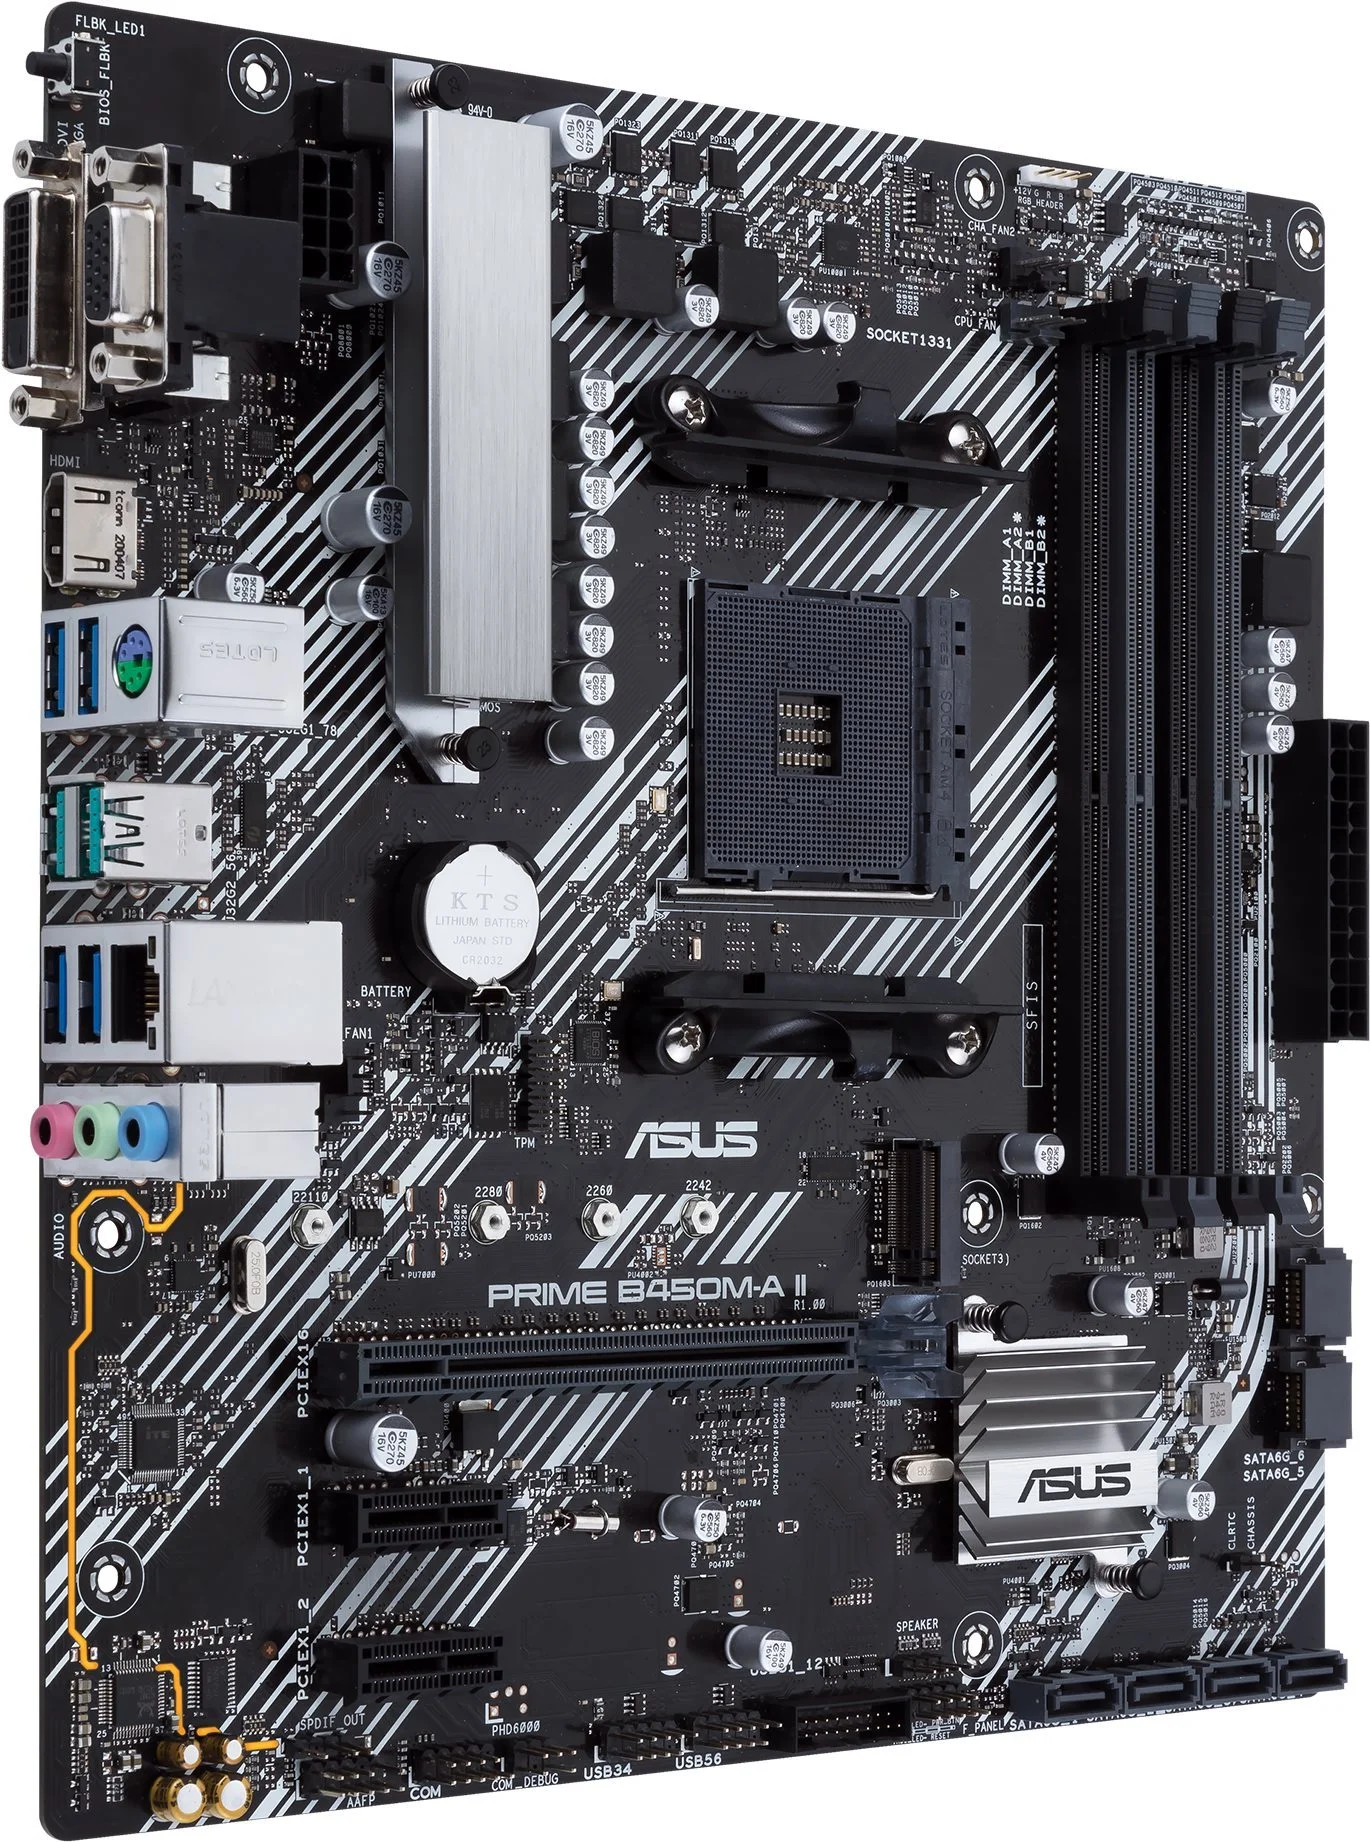
\includegraphics[scale=0.15]{./images/motherboard.png} % mozno pouzit scale=0.5
	\centering
	\caption{Základná doska - ASUS PRIME B450M-A II \\ Zdroj: https://www.alza.sk/asus-prime-b450m-a-ii-d6219596.htm}
\end{figure}

%tabulka špecifikacii základnej dosky
\begin{table}[h]
\centering
\begin{tabularx}{\linewidth}{|l|X|}
\hline
\textbf{Parameter} & \textbf{Hodnota} \\ \hline
Socket & AMD AM4 \\ \hline
Čipset & AMD B450 \\ \hline
Formát základnej dosky & mATX (Micro ATX) \\ \hline
Základné funkcie & Integrovaná sieťová karta, Integrovaná zvuková karta, M.2, PCI Express 3.0, Príprava pre CPU s integrovaným GPU, Serial ATA III \\ \hline
Typ slotov & DIMM \\ \hline
Typ pamäte & DDR4 \\ \hline
Počet slotov RAM & 4 × \\ \hline
Maximálna frekvencia (OC) & 4 400 MHz \\ \hline
Typ zvukovej karty & Realtek ALC897 \\ \hline
Počet kanálov zvukovej karty & 8 \\ \hline
Externé konektory & DVI, HDMI, Jack, PS/2, RJ-45 (LAN) 1Gbps, USB 3.2 Gen 1, USB 3.2 Gen 2, VGA (D-Sub) \\ \hline
Interné konektory & COM header, M.2 Socket, RGB LED Header, S/PDIF header, Serial ATA III, TPM header, USB 2.0 header, USB 3.2 Gen 1 header \\ \hline
PCI Express x16 & 1× \\ \hline
PCI Express x1 & 2× \\ \hline
USB 3.2 Gen 1 (USB 3.0) & 4× \\ \hline
USB 3.1 (3.1 gen2) & 2× \\ \hline
M.2 sloty & 1× \\ \hline
Serial ATA III & 6× \\ \hline
\end{tabularx}
\caption{Špecifikácie základnej dosky ASUS PRIME B450M-A II}
\end{table}

\subsection{Procesor}
Vybral som procesor AMD Ryzen 5 4600G, ktorý je dostatočne výkonný pre náš systém NAS. Procesor obsahuje 6 jadier a 12 vlákien s relatívne vysokou frekvenciou. Taktiež obsahuje integrovanú grafickú kartu, čo nám umožní ušetriť peniaze na samostatnej grafickej karte. Taktiež obsahuje chladič s dostatočnou chladiacou kapacitou pre naše využitie, ktorý nám ušetrí ďalšie náklady.

% obrazok procesora
\begin{figure}[H]
	\centering
	\captionsetup{justification=centering,margin=2cm}
	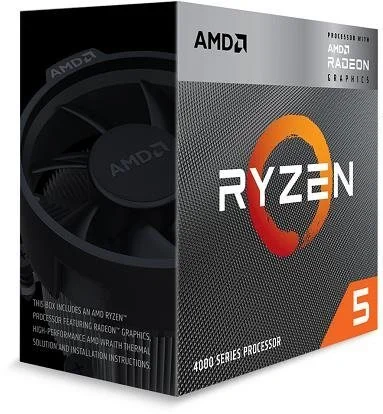
\includegraphics[scale=0.5]{./images/cpu.png} % mozno pouzit width=\linewidth
	\centering
	\caption{Procesor - AMD Ryzen 5 4600G \\ Zdroj: https://www.alza.sk/amd-ryzen-5-4600g-d7463833.htm}
\end{figure}

%tabulka špecifikacii procesora
\begin{table}[h]
\centering
\begin{tabularx}{\textwidth}{|l|X|}
\hline
\textbf{Parameter} & \textbf{Hodnota} \\ \hline
Rad procesora & AMD Ryzen 5 \\ \hline
Socket & AMD AM4 \\ \hline
Modelové označenie & AMD Ryzen 5 4600G \\ \hline
Mikroarchitektúra & Zen 2 \\ \hline
Počet jadier procesora & 6 × \\ \hline
Počet vláken & 12 × \\ \hline
Frekvencia procesora & 3,7 GHz (3,7 GHz) \\ \hline
Maximálna frekvencia (OC) & 4,2 GHz (4 200 MHz) \\ \hline
Podporovaný typ pamäte & DDR4 \\ \hline
Maximálny počet kanálov & 2 × \\ \hline
Typ integrovanej grafickej karty & AMD Radeon Graphics \\ \hline
Frekvencia integrovanej grafickej karty & 1 900 MHz \\ \hline
Funkcie & Automatické pretaktovanie, Virtualizácia, Integrované GPU, Multi-Threading, Chladič v balení \\ \hline
TDP & 65 W \\ \hline
Výrobné technológie & 7 nm \\ \hline
L2 cache & 3 MB \\ \hline
L3 cache & 8 MB \\ \hline
\end{tabularx}
\caption{Špecifikácie procesora AMD Ryzen 5 4600G}
\end{table}

\subsection{Pamäť}
Pre naše potreby použijeme 16 GB operačnej pamäte RAM. Je to viac než dosť a bude nám to tvoriť rezervu do budúcna. Vybral som dva moduly Kingston Fury s kapacitou 8 GB a frekvenciou 3200 MHz (2x8GB). Pamäť síce nie nemá funkcionalitu ECC\footnote{Error-correcting code}, avšak potom by sme potrebovali oveľa drahšiu základnú dosku a procesor, ktoré túto funkcionalitu podporujú.

% obrazok pamäte
\begin{figure}[H]
	\centering
	\captionsetup{justification=centering,margin=2cm}
	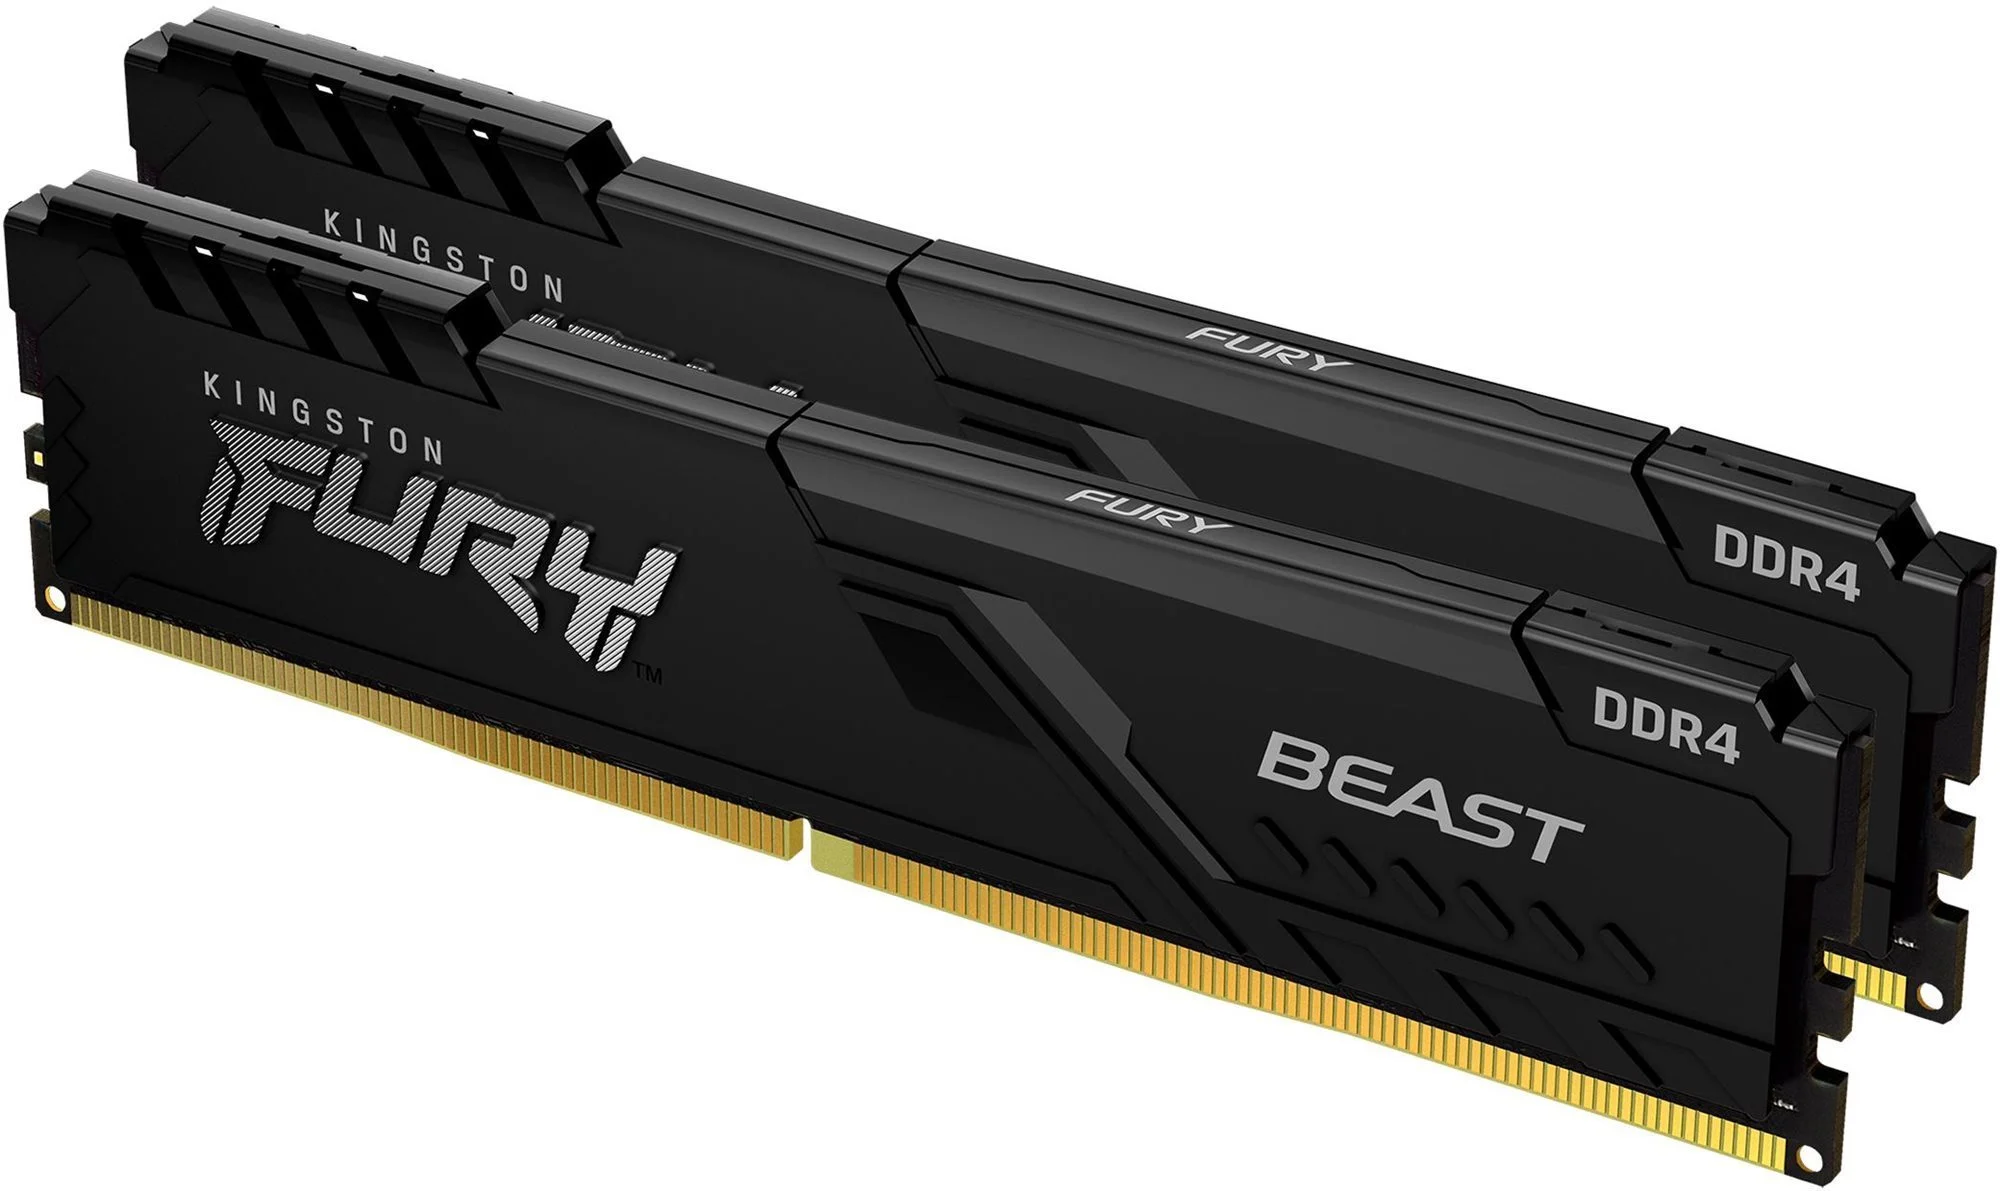
\includegraphics[scale=0.15]{./images/ram.png} % mozno pouzit width=\linewidth
	\centering
	\caption{Pamäť - Kingston FURY 16 GB KIT DDR4 3200 MHz CL16 Beast Black \\ Zdroj: https://www.alza.sk/kingston-fury-16-gb-kit-ddr4-3200-mhz-cl16-beast-black-d6622616.htm}
\end{figure}

%tabulka špecifikacii pamäte
\begin{table}[h]
\centering
\begin{tabularx}{\textwidth}{|l|X|}
\hline
\textbf{Parameter} & \textbf{Hodnota} \\ \hline
Určenie & Pre počítač \\ \hline
Vyhotovenie & DIMM \\ \hline
Typ pamäte & DDR4 \\ \hline
Modul pamäte & PC4-25600 \\ \hline
Veľkosť operačnej pamäte RAM & 16 GB \\ \hline
Počet modulov v balení & 2 ks \\ \hline
Moduly v balení & 2x8GB \\ \hline
Frekvencia pamäte & 3 200 MHz \\ \hline
Časovanie & CL16 \\ \hline
Časovanie & 16-18-18 \\ \hline
Priepustnosť & 25 600 MB/s \\ \hline
Napätie & 1,35 V \\ \hline
Ďalšie vlastnosti & Single Rank \\ \hline
Farba podsvietenia & Bez podsvietenia \\ \hline
RGB ovládanie & Nepodporuje \\ \hline
\end{tabularx}
\captionsetup{justification=centering,margin=2cm}
\caption{Špecifikácie pamäte Kingston FURY 16 GB KIT DDR4 3200 MHz CL16 Beast Black}
\end{table}

\subsection{Disky}
Náš systém bude potrebovať okrem dátových diskov aj disk, kde bude uložený samotný operačný systém (bootovací disk). Na tento účel nám bude slúžiť práve SSD disk, ktorý bude umiestnený v M.2 slote na základnej doske.

\subsubsection{Bootovací disk}
Ako bootovací disk nám bude bohate postačovať Patriot P300 s veľkosťou 128GB. Disk má rozhranie PCIe verzie 3.0 čo je síce starší štandard ale na naše potreby bude stačiť a naša základná doska aj tak nepodporuje novší štandard. Veľkosť disku prekračuje potreby operačného systému ale keďže ide o veľmi lacnú položku, tak sa neoplatí kupovať nejaký nespoľahlivý USB disk s menšou kapacitou alebo SD kartu. Radšej investujeme do kvalitného SSD disku ktorý nám bude slúžiť aj do budúcna.

% obrazok boot disku
\begin{figure}[H]
	\centering
	\captionsetup{justification=centering,margin=2cm}
	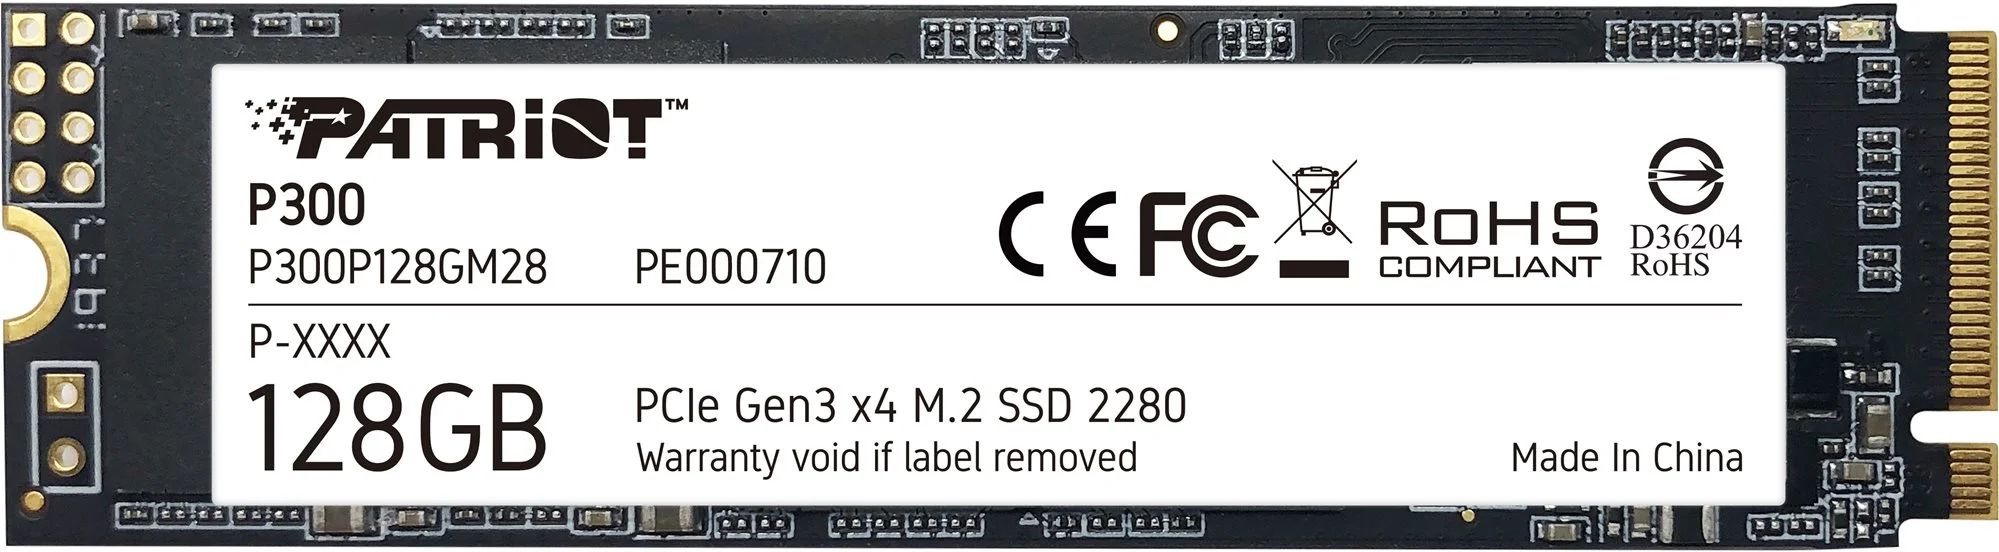
\includegraphics[scale=0.2]{./images/boot-drive.png} % mozno pouzit width=\linewidth
	\centering
	\caption{Bootovací disk - Patriot P300 128GB \\ Zdroj: https://www.alza.sk/patriot-p300-128gb-d5798224.htm}
\end{figure}

\pagebreak

%tabulka špecifikacii boot disku
\begin{table}[h]
\centering
\begin{tabularx}{\textwidth}{|l|X|}
\hline
\textbf{Parameter} & \textbf{Hodnota} \\ \hline
Kapacita úložiska (HDD + SSD) & 128 GB (0,13 TB) \\ \hline
Typ úložiska & SSD \\ \hline
Formát (Form Factor) & M.2 \\ \hline
Kapacita disku & 128 GB (0,13 TB) \\ \hline
Šírka & 22 mm (2,2 cm) \\ \hline
Výška & 3,8 mm (0,38 cm) \\ \hline
Hĺbka & 80 mm (8 cm) \\ \hline
Hmotnosť & 20 g (0,02 kg) \\ \hline
Farba & Čierna \\ \hline
Rad disku & Patriot P300 \\ \hline
Použitie & Do počítača, Do notebooku, Interný \\ \hline
Rozhranie interné & M.2 (PCIe 3.0 4x NVMe) \\ \hline
Rýchlosť náhodného čítania & 290 000 IOPS \\ \hline
Rýchlosť náhodného zápisu & 150 000 IOPS \\ \hline
Rýchlosť čítania & 1 600 MB/s \\ \hline
Rýchlosť zápisu & 600 MB/s \\ \hline
Radič & Silicon Motion SM2263XT \\ \hline
Veľkosť článku/bunky & TLC (Triple-Level Cell) \\ \hline
Životnosť disku & 40 TBW \\ \hline
Typická spotreba & 2,07 W \\ \hline
Stand-by spotreba (pohotovostná) & 0,37 W (370 mW) \\ \hline
\end{tabularx}
\caption{Špecifikácie SSD disku Patriot P300 128GB}
\end{table}


\subsubsection{Dátové disky}
Pri výbere dátových diskov (najdôležitejšou časťou pre nás) som zohľadniľ internetové recenzie a moje doterajšie znalosti. Rozhodoval som sa medzi WD Red Pro a Seagate IronWolf Pro. Nakoniec som zvolil Seagate IronWolf Pro pretože boli viacej doporučované na internete a majú väčšiu vyrovnávaciu pamäť (cache) čo nám zvýši rýchlosť pri čítaní a zápise dát. Zvolil som 2 TB verziu pretože na naše účely by to bolo dostatočné. Keďže pôjde o 4 disky, tak nám to dáva celkovú kapacitu 8 TB. Ale kvôli použitiu redundancie nám ostanú ``len'' 4 TB reálneho miesta.

% obrazok data disku
\begin{figure}[H]
	\centering
	\captionsetup{justification=centering,margin=2cm}
	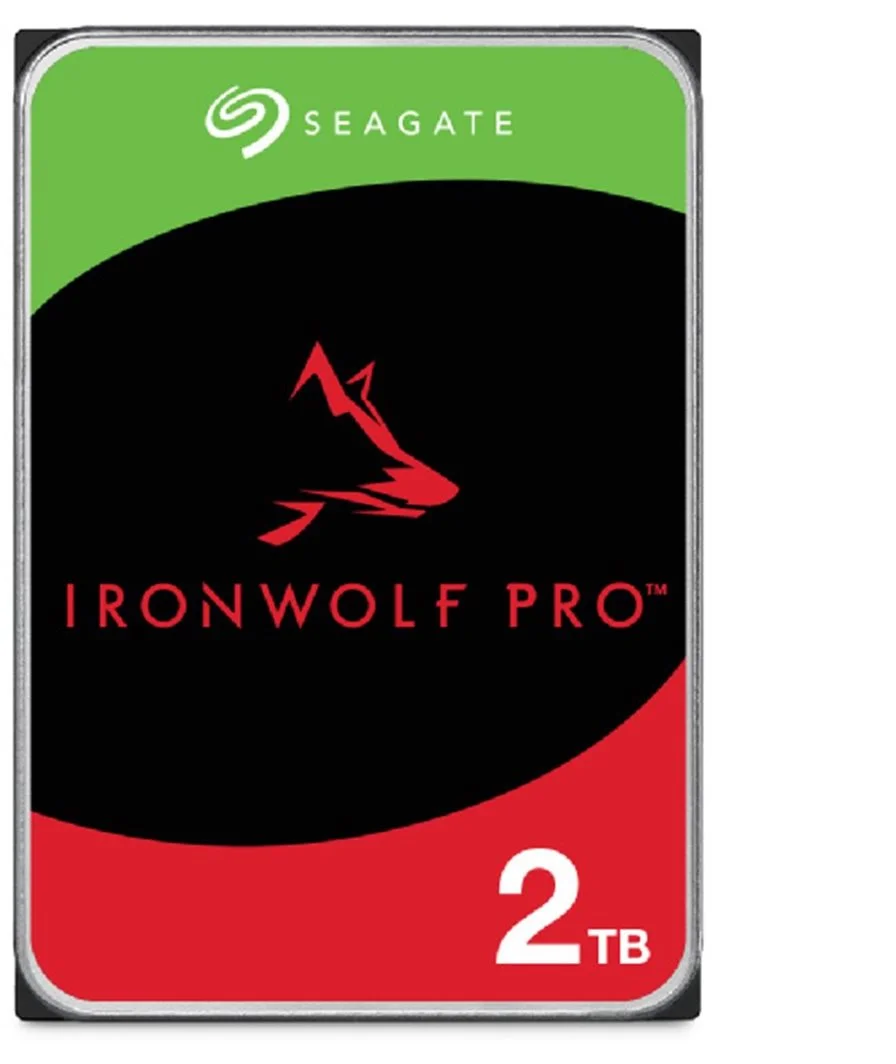
\includegraphics[scale=0.2]{./images/data-drive.png} % mozno pouzit width=\linewidth
	\centering
	\caption{Dátový disk - Seagate IronWolf Pro 2 TB \\ Zdroj: https://www.alza.sk/seagate-ironwolf-pro-2-tb-d7470754.htm}
\end{figure}

%tabulka špecifikacii data disku
\begin{table}[h]
\centering
\begin{tabularx}{\textwidth}{|l|X|}
\hline
\textbf{Parameter} & \textbf{Hodnota} \\ \hline
Kapacita úložiska (HDD + SSD) & 2 000 GB (2 TB) \\ \hline
Typ úložiska & HDD \\ \hline
Formát (Form Factor) & 3.5" \\ \hline
Kapacita disku & 1 953,13 GB (1,91 TB) \\ \hline
Šírka & 101,85 mm (10,19 cm) \\ \hline
Výška & 26,11 mm (2,61 cm) \\ \hline
Hĺbka & 146,99 mm (14,7 cm) \\ \hline
Hmotnosť & 620 g (0,62 kg) \\ \hline
Farba & Čierna, Červená \\ \hline
Rad disku & Seagate IronWolf Pro \\ \hline
Použitie & Do počítača, Dátové úložiská, Interný \\ \hline
Rozhranie interné & SATA III \\ \hline
Rýchlosť čítania & 226 MB/s \\ \hline
Rýchlosť zápisu & 226 MB/s \\ \hline
Technológia zápisu & CMR \\ \hline
Vyrovnávacia pamäť & 256 MB \\ \hline
Radič & Seagate \\ \hline
Maximálna hlučnosť & 30 dB(A) \\ \hline
Mean Time Before Failure & 2 000 000 h \\ \hline
Typická spotreba & 6,7 W \\ \hline
Stand-by spotreba (pohotovostná) & 1 W (1 000 mW) \\ \hline
\end{tabularx}
\caption{Špecifikácie dátového disku Seagate IronWolf Pro 2TB}
\end{table}

\subsection{Zdroj napájania}
Ako zdroj napájania by nám stačil aj 3OO/350W zdroj avšak kvôli rezerve a vysokej účinnosti som sa rozhodol pre zdroj s výkonom 400W. Vybral som zdroj Be quiet! PURE POWER 11 400 W. Zdroj má vysokú účinnosť a tichý chod, čo je pre pre nás dôležité keďže bude umiestnený v byte a bude bežať nonstop (24/7). Taktiež má dostatok káblov pre všetky možné disky.

% obrazok zdroja
\begin{figure}[H]
	\centering
	\captionsetup{justification=centering,margin=2cm}
	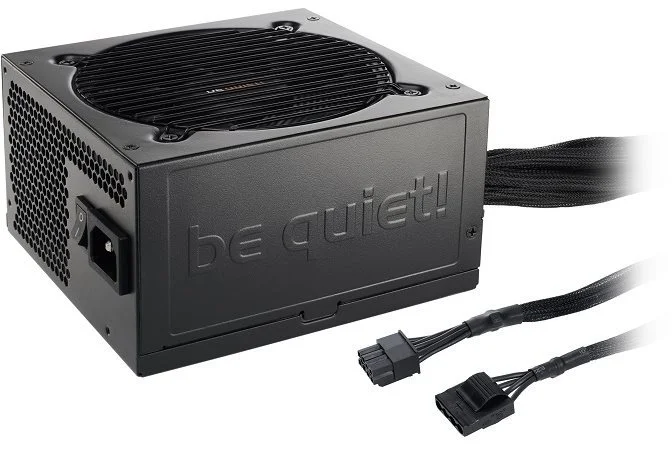
\includegraphics[scale=0.5]{./images/power-supply.png} % mozno pouzit width=\linewidth
	\centering
	\caption{Zdroj napájania - Be quiet! PURE POWER 11 400 W \\ Zdroj: https://www.alza.sk/be-quiet-pure-power-11-400w-d5549562.htm}
\end{figure}

%tabulka špecifikacii zdroja
\begin{table}[h]
\centering
\begin{tabularx}{\textwidth}{|l|X|}
\hline
\textbf{Parameter} & \textbf{Hodnota} \\ \hline
Výkon & 400 W \\ \hline
Formát & ATX \\ \hline
Verzia & ATX 2.4 \\ \hline
Výbava a funkcie & Aktivny PFC, Tepelná regulácia otáčok, Sieťový vypínač \\ \hline
Typ ochrany & Podpäťová ochrana, Nadprúdová ochrana (OCP), Ochrana proti preťaženiu (OPP), Ochrana proti skratu (SCP), Ochrana proti prehriatiu (OTP) \\ \hline
Certifikácia & 80 PLUS Gold \\ \hline
Účinnosť & 92 \% \\ \hline
Konektory & ATX 24pin, CPU 8pin / 4+4pin, Floppy 4pin, Molex 4pin, PCI-E 8pin / 6+2pin, SATA 15pin \\ \hline
Počet PCI Express 8-pin & 2× \\ \hline
Počet Serial ATA 15-pin & 5× \\ \hline
Počet Molex HDD 4-pin & 2× \\ \hline
Počet Molex FDD 4-pin & 1× \\ \hline
Veľkosť ventilátora & 120 mm \\ \hline
Maximálna hlučnosť & 14,9 dB \\ \hline
Šírka & 150 mm (15 cm) \\ \hline
Výška & 150 mm (15 cm) \\ \hline
Hĺbka & 86 mm (8,6 cm) \\ \hline
Hmotnosť & 1,93 kg (1 930 g) \\ \hline
\end{tabularx}
\caption{Špecifikácie zdroja Be quiet! PURE POWER 11 400 W}
\end{table}

\subsection{Kabeláž}
Na prepojenie nášho systému NAS a nášho domáceho PC použijeme tienený (FTP) CAT6 kábel s dĺžkou 15 metrov. Tento kábel je vhodný pre gigabitové siete a je odolný voči prípadnému elektromagnetickému rušeniu. Taktiež budeme potrebovať káble pre pripojenie dátových diskov. Na to použijeme SATA káble ktoré sú súčasťou balenia základnej dosky. Keďže sa tam nachádzajú iba dva káble, tak budeme musieť dokúpiť ďalšie dva.

% obrazok FTP kabla
\begin{figure}[H]
	\centering
	\captionsetup{justification=centering,margin=2cm}
	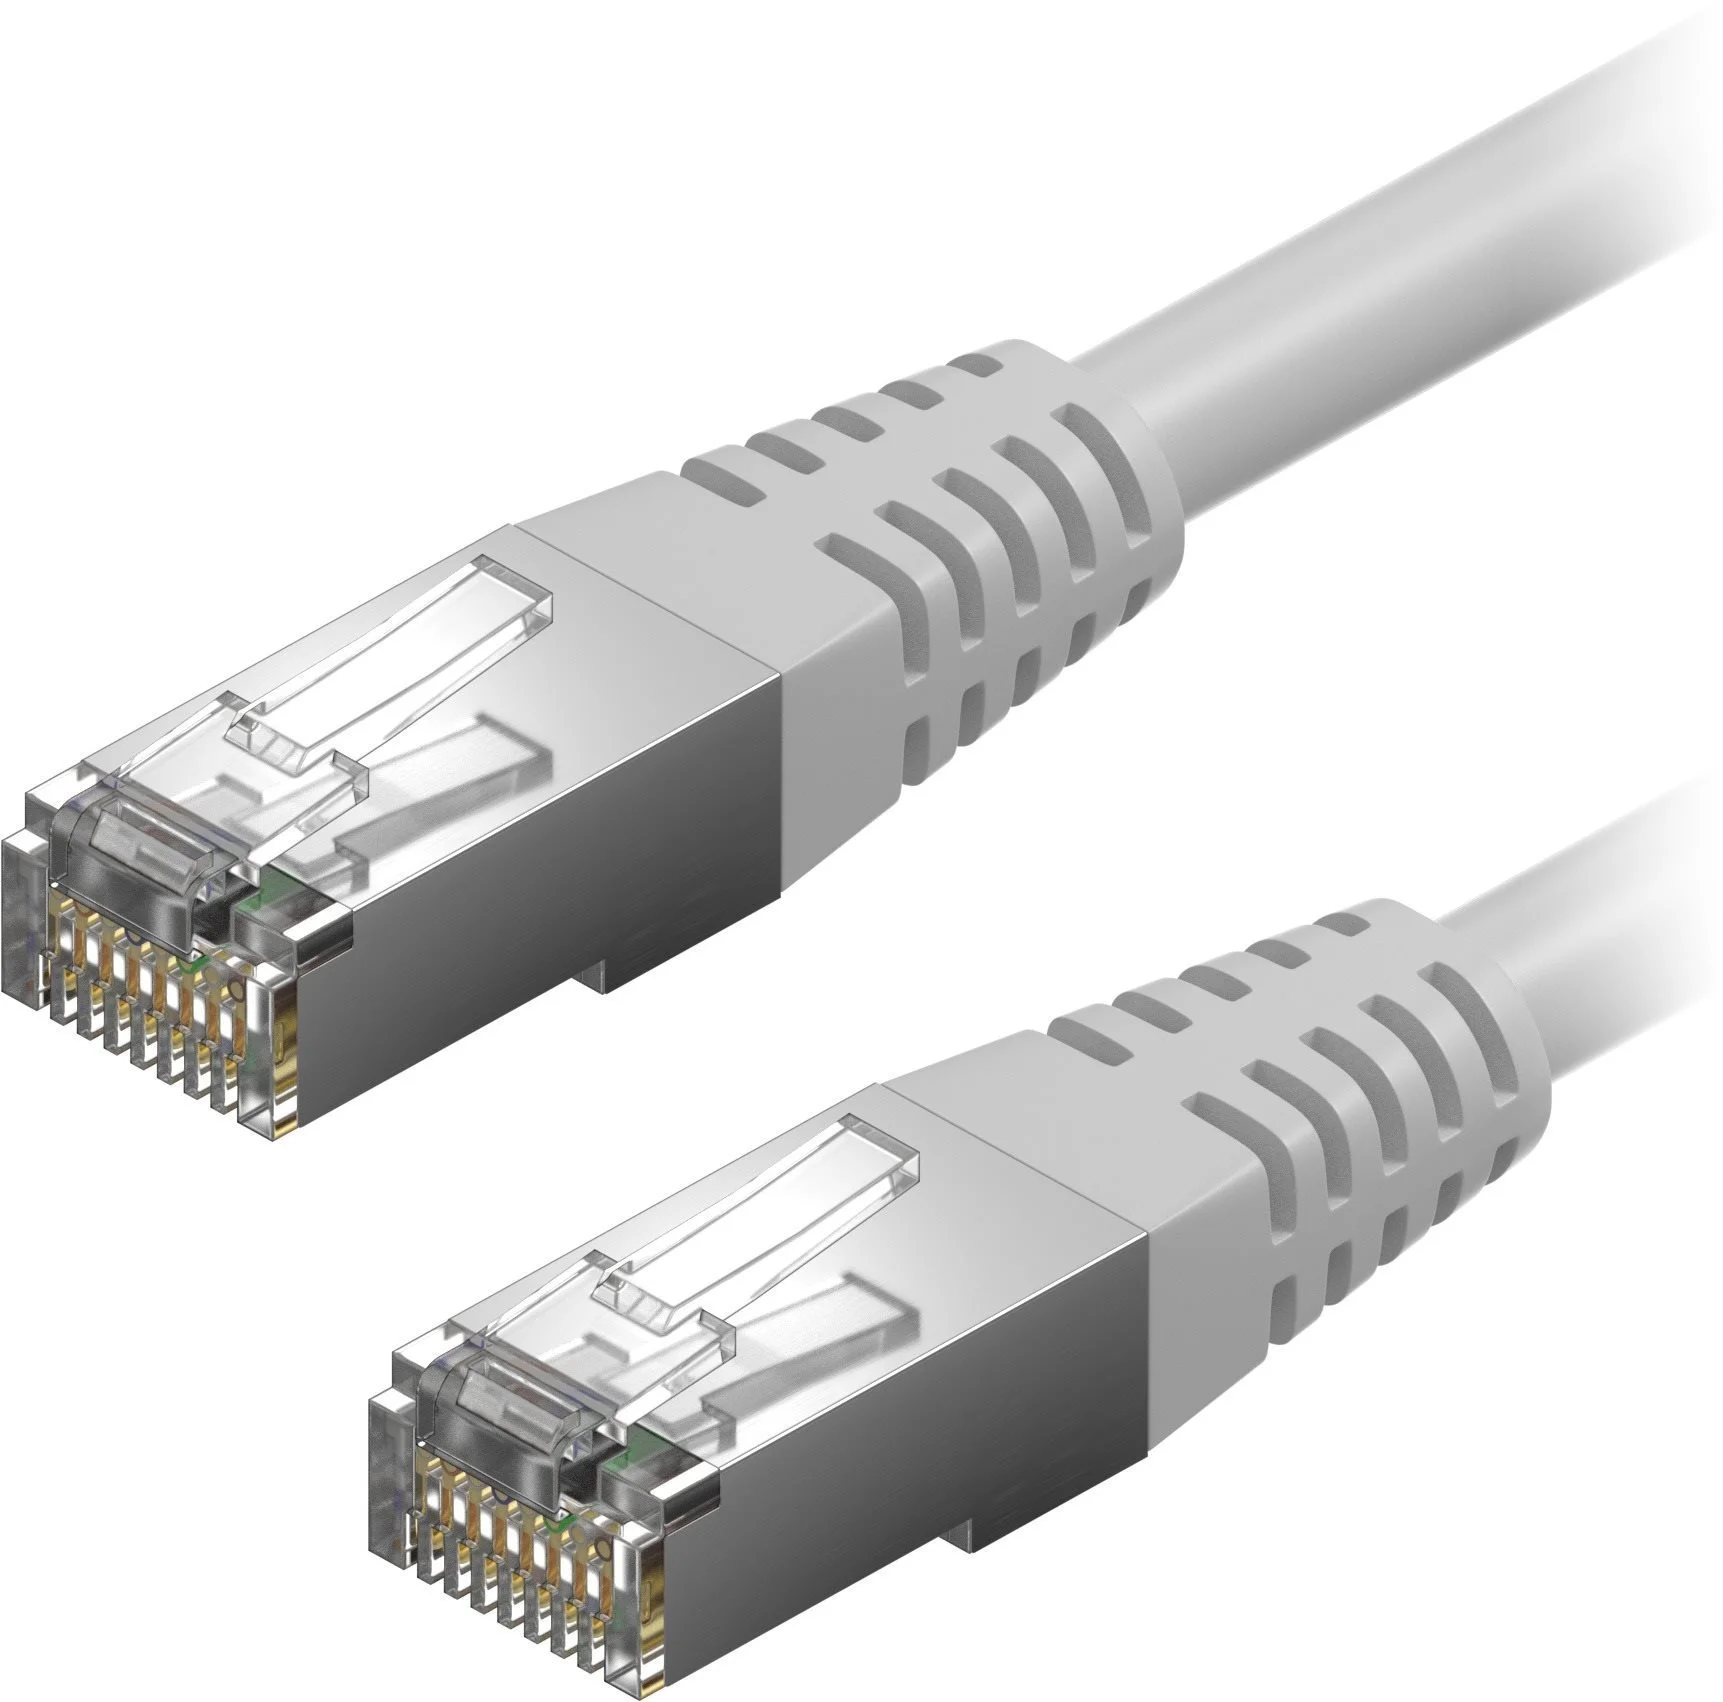
\includegraphics[scale=0.1]{./images/ftp.png} % mozno pouzit width=\linewidth
	\centering
	\caption{Sieťový kábel - AlzaPower Patch CAT6 FTP 15 m \\ Zdroj: https://www.alza.sk/alzapower-patch-cat6-ftp-15-m-sivy-d6592195.htm}
\end{figure}

%tabulka špecifikacii FTP kabla
\begin{table}[h]
\centering
\begin{tabular}{|l|l|}
\hline
\textbf{Parameter} & \textbf{Hodnota} \\ \hline
Typ & Prepojovací kábel \\ \hline
Male konektor - Typ & RJ-45 \\ \hline
Male konektor - Štandard & CAT6 \\ \hline
Male konektor - Počet & 2 × \\ \hline
Dĺžka kábla & 15 m \\ \hline
Zakončenie & Rovné \\ \hline
Tienenie & FTP \\ \hline
Vlastnosti & Obojstranná koncovka, Tienený kábel \\ \hline
Farba & Sivá \\ \hline
\end{tabular}
\caption{Špecifikácie sieťového kábla}
\end{table}

% obrazok SATA kabla
\begin{figure}[H]
	\centering
	\captionsetup{justification=centering,margin=2cm}
	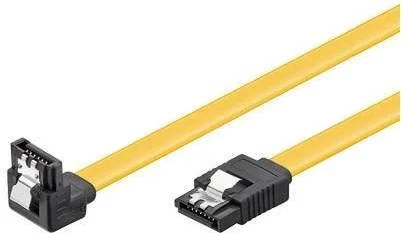
\includegraphics[scale=0.4]{./images/sata.png} % mozno pouzit width=\linewidth
	\centering
	\caption{SATA kábel - PremiumCord SATA III 90° 0.2 m \\ Zdroj: https://www.alza.sk/premiumcord-sata-iii-90-0-2m-d2147595.htm}
\end{figure}

%tabulka špecifikacii SATA kabla
\begin{table}[h]
\centering
\begin{tabular}{|l|l|}
\hline
\textbf{Parameter} & \textbf{Hodnota} \\ \hline
Typ & Prepojovací kábel \\ \hline
Male konektor - Typ & SATA \\ \hline
Male konektor - Štandard & Serial ATA III \\ \hline
Male konektor - Počet & 2 × \\ \hline
Dĺžka kábla & 0,2 m \\ \hline
Zakončenie & Zahnuté \\ \hline
Vlastnosti & Obojstranná koncovka \\ \hline
Farba & Žltá \\ \hline
\end{tabular}
\caption{Špecifikácie prepojovacieho kábla}
\end{table}



\section{Softvér}
Zo softvérovej časti je treba si zvoliť aký typ redundancie dát chceme, aký operačný systém použijeme pre náš projekt.

\subsection{RAID}
RAID\footnote{Redundant Array of Independent Disks} je metóda, ktorá nám umožňuje kombinovať viacero diskov do jedného logického celku. Jednotlivé typy polí dosahujú v závislosti od konfigurácie rôznu úroveň zabezpečenia dát pred chybami a stratou spôsobenou zlyhaním hardvéru a rôzne veľké zvýšenie výkonu (dátovej priepustnosti) pri diskových operáciách vo vzťahu k počtu diskov, potrebe špecializovaných radičov polí a tým aj cene riešenia.

RAID má viacero typov, ktoré sa líšia v počte diskov, ktoré môžu zlyhať aby nám nevznikla strata dát. Typy RAIDov:
\begin{spacing}{1.0}
    \begin{itemize}
        \item RAID 0
            \begin{itemize}
                \item Dáta sú rozdelené medzi viaceré disky pre zvýšenie rýchlosti, ale neponúka žiadnu redundanciu dát. Ak zlyhá jeden disk, prídeme o všetky dáta.
            \end{itemize}
        \item RAID 1
            \begin{itemize}
                \item Dáta sú zrkadlené na dvoch diskoch pre úplnú redundanciu dát. Môžeme prísť o jeden disk.
            \end{itemize}
        \item RAID 5
            \begin{itemize}
                \item Používa jeden disk na paritné dáta. Dáta a parita sú rozdelené medzi tri alebo viac diskov. Poskytuje toleranciu chýb pri zlyhaní jedného disku.
            \end{itemize}
        \item RAID 6
            \begin{itemize}
                \item Podobné ako RAID 5, ale používa dva paritné disky, čo ponúka extra redundanciu dát. Z toho vyplýva že môžeme prísť až o dva disky, ale potrebujeme minimálne 4 disky.
            \end{itemize}
        \item RAID 10
            \begin{itemize}
                \item Kombinuje RAID 0 a RAID 1. Poskytuje redundanciu RAID 1 spolu so zvýšeným výkonom RAID 0.
            \end{itemize}
    \end{itemize}
\end{spacing}

Rozhodol som sa, že v našom projekte použijeme RAID 6 ktorý nám zaručuje vysokú redundaciu dát (môžeme prísť až o dva disky) avšak za cenu toho že z celkovej kapacity diskov nám ostane len 50\% (pri 4 diskoch). Nič nám však nebráni v prípade potreby použiť až 6 diskov keďže nám to naša PC skriňa umožnuje. Týmto vieme zvýšiť celkovú reálnu kapacitu.

% obrazok RAID 6
\begin{figure}[H]
	\centering
	\captionsetup{justification=centering,margin=2cm}
	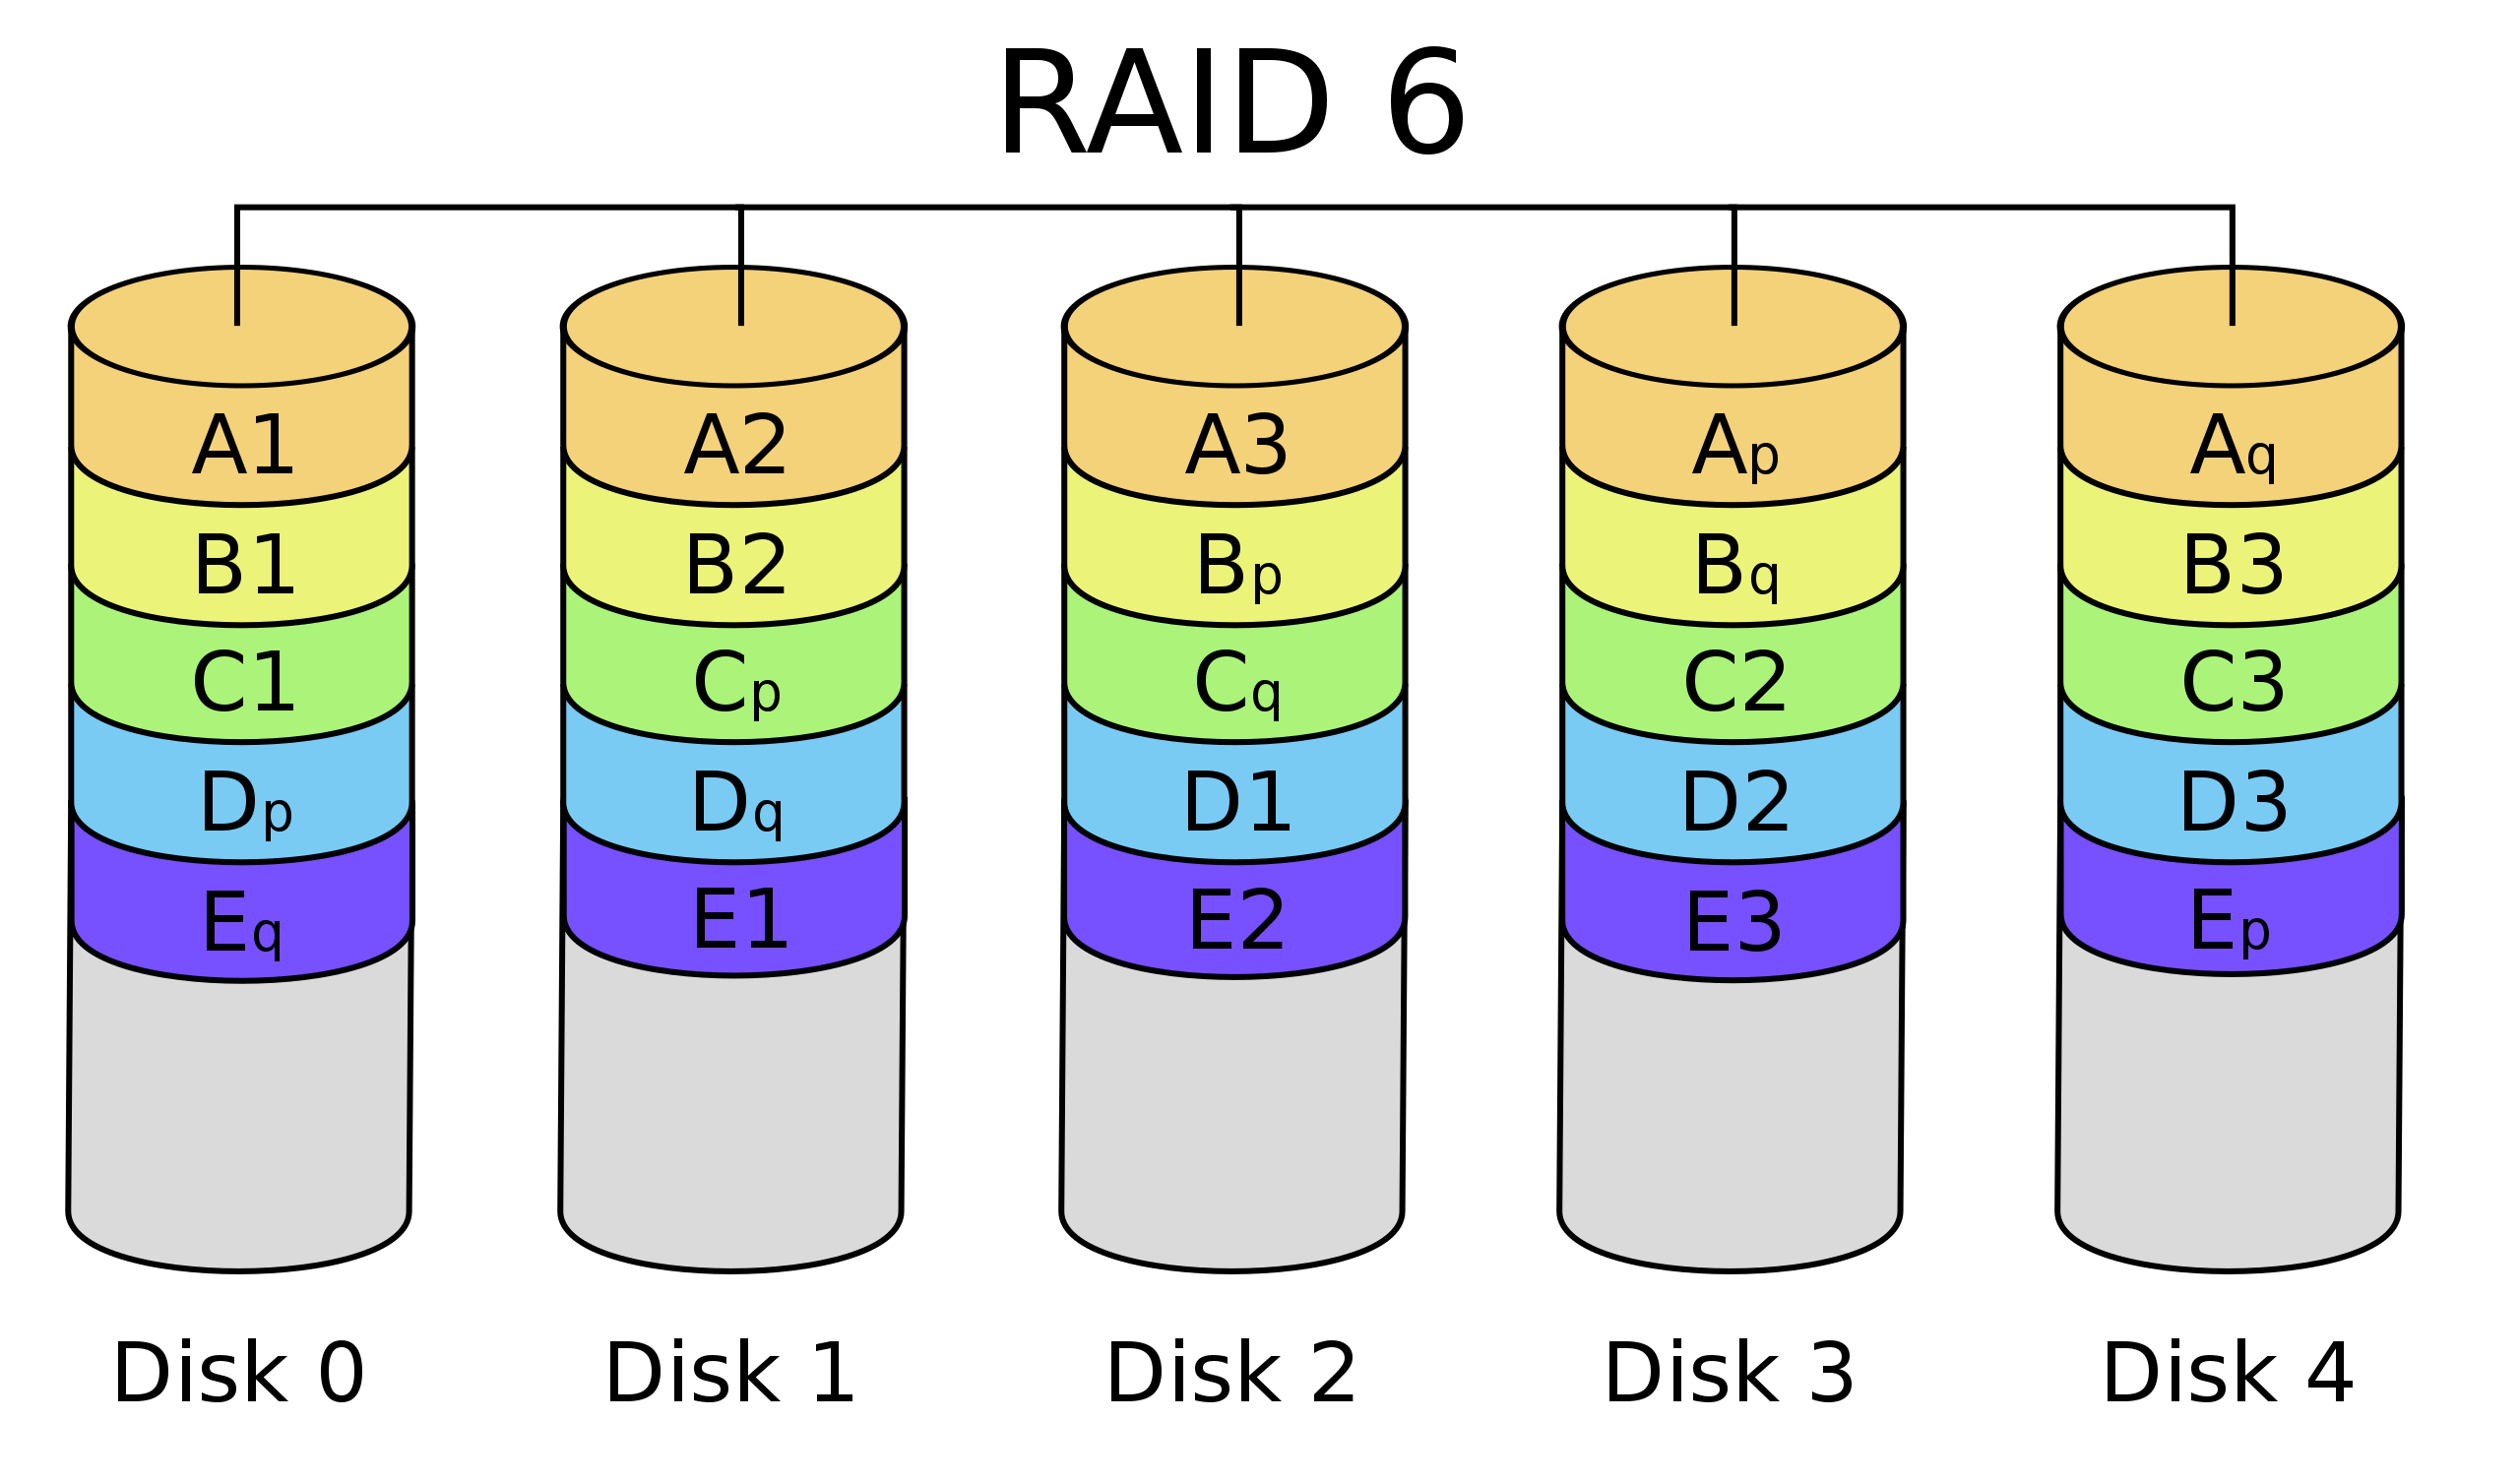
\includegraphics[width=\linewidth]{./images/RAID_6.png} % mozno pouzit width=\linewidth
	\centering
	\caption{RAID 6 \\ Zdroj: https://sk.wikipedia.org/wiki/RAID}
\end{figure}

\subsection{Operačný systém}
Rozhodoval som sa medzi dvomi operačnými systémami TrueNAS a OpenMediaVault. Podľa internetových recenzií a svojho uváženia som sa rozhodol pre OpenMediaVault. TrueNAS je síce viac profesionálny a podporuje veľa funkcií ale pre naše potreby je OpenMediaVault viac než dostatočný. Je to open-source projekt, čo znamená že má dostupný zdrojový kód a môžeme si ho prispôsobiť podľa našich potrieb.

OpenMediaVault je primárne určený na používanie v domácom prostredí alebo malých domácich kanceláriách, ale nie je obmedzený len na tieto scenáre. Je to jednoduché a ľahko použiteľné riešenie, ktoré môže nainštalovať a spravovať každý bez toho, aby potreboval znalosti na úrovni experta v oblasti sieťových a dátových systémov.

Systém je postavený na modulárnej konštrukcii a možno ho ľahko rozšíriť pomocou pluginov dostupných hneď po inštalácii základného systému. Ďalšie pluginy tretích strán sú k dispozícii prostredníctvom repozitára OMV-Extras.

Kedže máme veľmi výkonný stroj, tak si vieme nainštalovať plugin Plex Media Server. Tento multimediálny server slúži na lokálne streamovanie filmov uložených na našom systéme NAS. Kedže budeme lokálne dekódovať filmy, tak náš výkonejší procesor nám zaručí plynulé prehrávanie aj pri vyšších rozlíšeniach.

% obrazok OpenMediaVault
\begin{figure}[H]
	\centering
	\captionsetup{justification=centering,margin=2cm}
	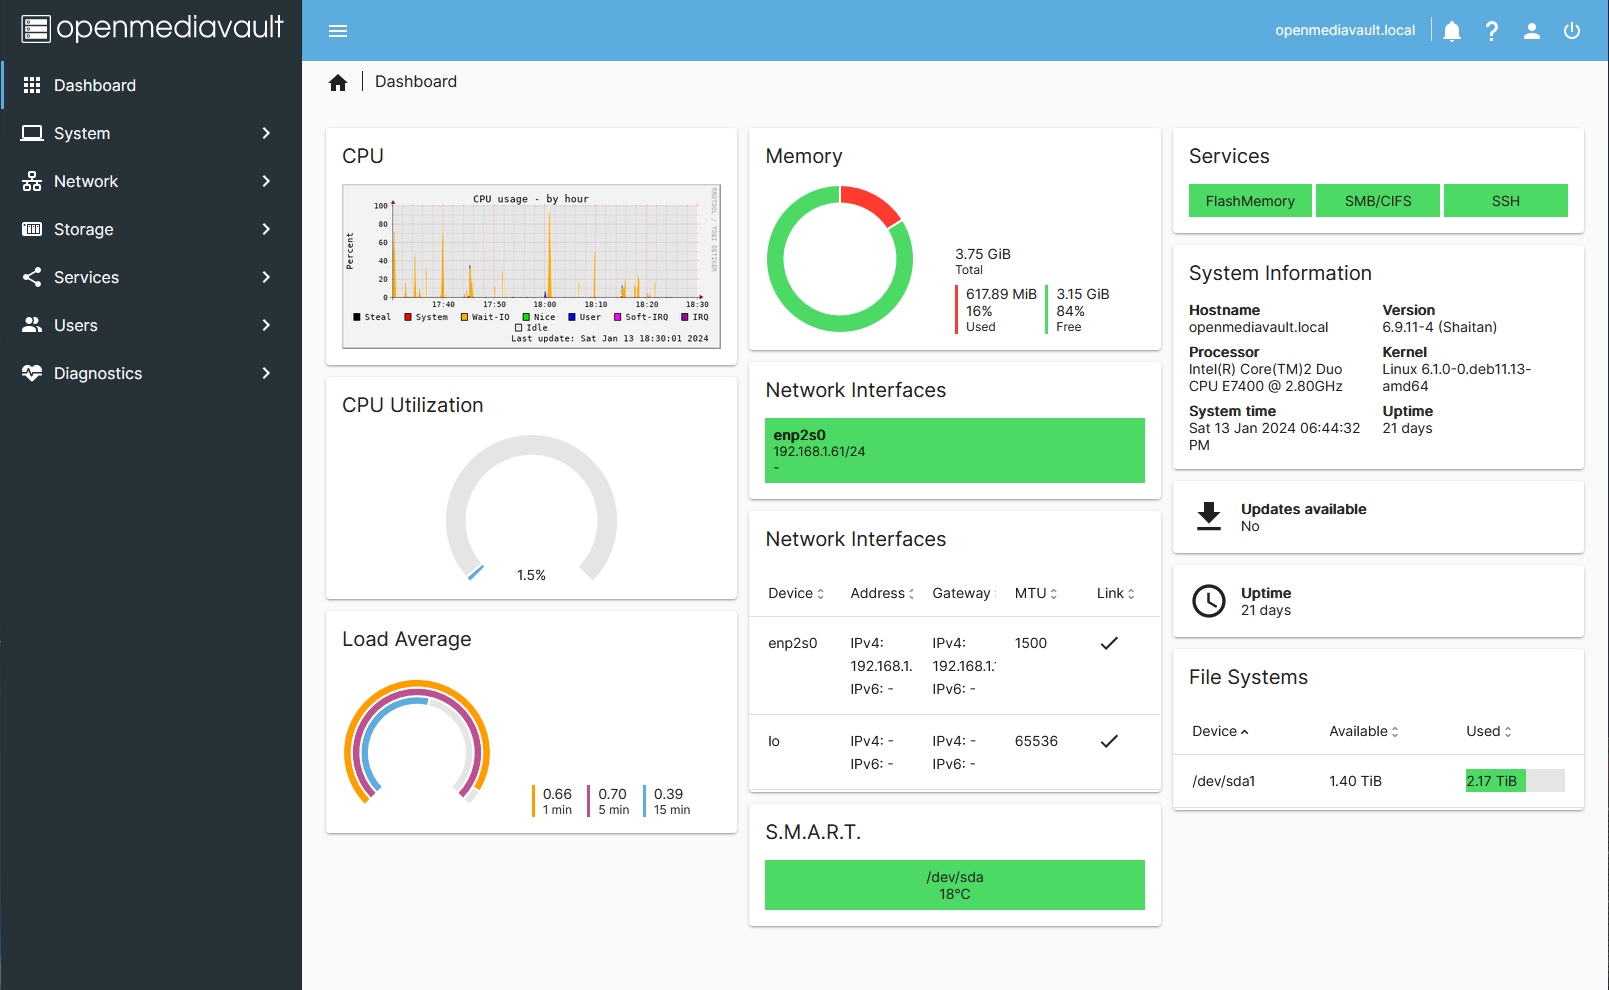
\includegraphics[width=\linewidth]{./images/OMV6_dashboard.png} % mozno pouzit width=\linewidth
	\centering
	\caption{Ukážka používateľského rozhrania OMV \\ Zdroj: https://en.wikipedia.org/wiki/OpenMediaVault}
\end{figure}

\section{Umiestnenie v domácnosti}
Keďže ide o domáci NAS, ktorý by som sám používal, zameral som sa na umiestnenie v byte, ktoré by bolo pre mňa najvhodnejšie z pohľadu hlučnosti. Rozhodol som sa umiestniť NAS pod stôl v pracovni, kde by nebol počuť, ale zároveň by bol k nemu dobrý prístup. Môžeme si to všimnúť na zjednodušenom pôdoryse[\ref{fig:floorplan}] bytu.

Legenda:
\begin{spacing}{1.0}
\begin{itemize}
	\item \textcolor{green}{Router}
	\item \textcolor{red}{NAS}
	\item \textcolor{blue}{Sieťová kabeláž vedúca cez rohovú lištu}
	\item \textcolor{orange}{Domáci počítač}
\end{itemize}
\end{spacing}

\begin{figure}[H]
	\centering
	\captionsetup{justification=centering,margin=2cm}
	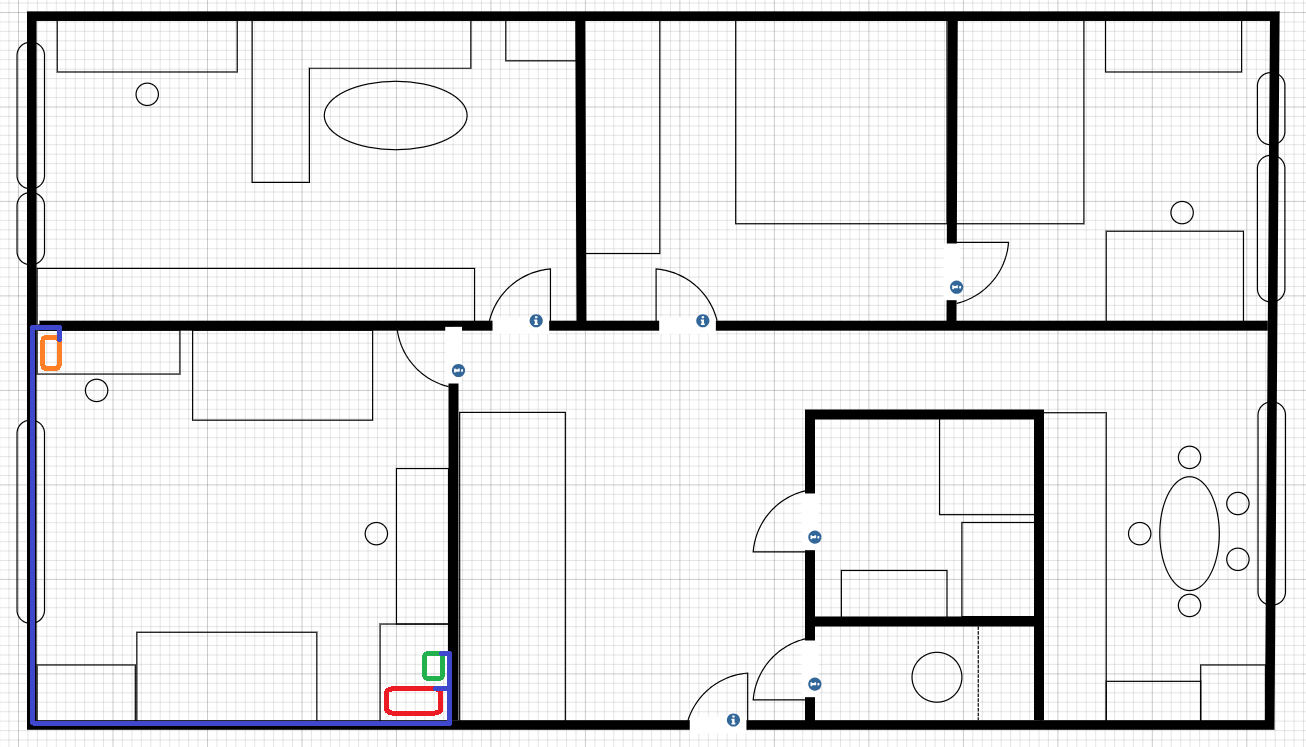
\includegraphics[width=\linewidth]{./images/nakres-bytu.png}
	\centering
	\caption{Pôdorys bytu}
	\label{fig:floorplan}
\end{figure}


\section{Porovnanie s inými riešeniami}
Ako prvú máme tabuľku s cenami spoločných položiek pre všetky riešenia. Sú tam zahrnuté dátové disky a sieťová kábel z dôvodu, že pri všetkých riešeniach by sme tieto položky potrebovali a teda dáva zmysel ich vynechať z porovnania.

\begin{table}[h]
\centering
\begin{tabular}{|l|c|}
\hline
\textbf{Položka} & \textbf{Cena (€)} \\ \hline
Dátové disky & 4 x 113,90 \\ \hline
CAT6 FTP kábel & 8,99 \\ \hline
\textbf{Celková cena} & 465,19\\ \hline
\end{tabular}
\caption{Cena spoločných položiek}
\end{table}

\subsection{Moje riešenie}
Moje riešenie je založené na vysoko výkonných komponentoch a RAID 6 konfigurácii s operačným systémom OpenMediaVault, ktorý je zadarmo. Celková cena komponentov pre moje riešenie je 365,78 €.

\begin{table}[h]
\centering
\begin{tabular}{|l|c|}
\hline
\textbf{Položka} & \textbf{Cena (€)} \\ \hline
PC Skriňa & 65,90 \\ \hline
Základná doska & 76,90 \\ \hline
Procesor & 96,90 \\ \hline
Pamäť & 42,90 \\ \hline
Bootovací Disk & 15,90 \\ \hline
Zdroj & 61,90 \\ \hline
SATA káble & 2 x 2,69 \\ \hline
\textbf{Celková cena} & 365,78 \\ \hline
\end{tabular}
\caption{Cena komponentov pre moje riešenie}
\end{table}

\subsection{Komerčné riešenia}
Komerčné riešenia som všetky hľadal na internetovom obchode Alza.sk aby boli ceny jednodné, kedže všetky komponenty a ich ceny som vzal práve odtiaľto. Hľadal som systémy NAS s podobnými parametrami ako moje riešenie. Požiadavky boli aby mal systém aspoň 4 pozície pre dátové disky, výkonný procesor a aspoň 8 GB operačnej pamäte RAM. Kedže komerčné riešenia sú ale veľmi špecializované na tento účel, tak vačšina systémou mala slabšie ale zase efektívnejšie procesory (spotreba) a menej operačnej pamäte. Vybral som teda populárne riešenie Synology DS923+ ktoré stojí 689 €. Boli al lacnejšie riešenia ale mali veľmi slabé procesory.

\begin{figure}[H]
	\centering
	\captionsetup{justification=centering,margin=2cm}
	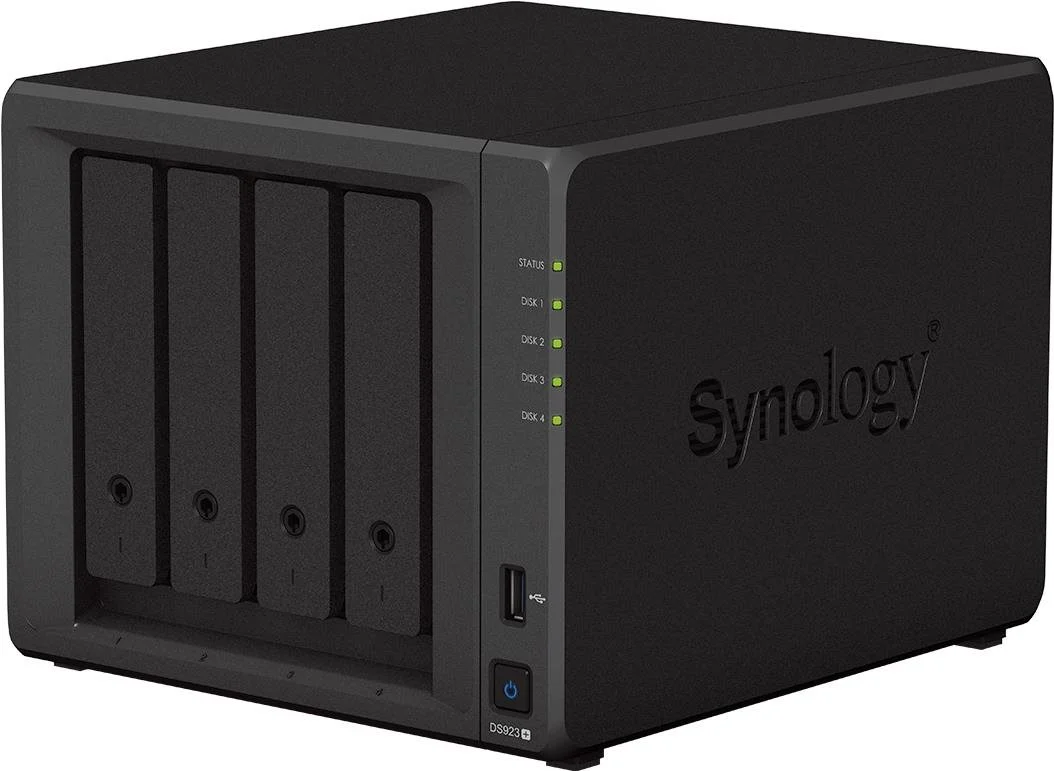
\includegraphics[scale=0.4]{./images/synology.png}
	\centering
	\caption{Synology DS923+ \\ Zdroj: https://www.alza.sk/synology-ds923-d7579640.htm}
\end{figure}

\begin{table}[h]
\centering
\begin{tabularx}{\textwidth}{|l|X|}
\hline
\textbf{Parameter} & \textbf{Hodnota} \\ \hline
Maximálna kapacita & 54 TB \\ \hline
Počet pozícií pre disk & 4 × \\ \hline
Počet pozícií osadených diskom & 0 × \\ \hline
Podporovaný RAID & RAID 5, RAID 6, RAID 0+1, RAID 10 (1+0), Špeciálny \\ \hline
Kompatibilný typ disku & 2,5" SATA HDD, 3,5" SATA HDD, M.2 NVMe \\ \hline
Podporované služby & Media server (DLNA), Zdieľanie súborov (SAMBA, HFS, CIFS), Nahrávanie z IP kamier, iSCSI, Print server \\ \hline
Systémová pamäť (RAM) & 3,91 GB (4 000 MB) \\ \hline
Typ pamäte & DDR4 \\ \hline
Pamäť RAM rozšíriteľná na & 31,25 GB (32 000 MB) \\ \hline
Frekvencia procesora & 3,1 GHz \\ \hline
Rýchlosť čítania & 592 MB/s \\ \hline
Rýchlosť zápisu & 562 MB/s \\ \hline
Procesor & AMD Ryzen R1600 \\ \hline
Využitie & Domáci, Firemný, Monitorovací systém \\ \hline
Vyhotovenie & Desktop \\ \hline
eSATA & 1 × \\ \hline
LAN & 2 × \\ \hline
USB 3.2 Gen 1 (USB 3.0) & 2 × \\ \hline
M.2 NVMe & 2 × \\ \hline
Spotreba v Stand-by & 11,52 W \\ \hline
Typická spotreba & 35 W \\ \hline
Hĺbka & 223 mm \\ \hline
Výška & 166 mm \\ \hline
Šírka & 199 mm \\ \hline
Hmotnosť & 2,24 kg \\ \hline
Obsah balenia & Balíček doplnkov × 1, Napájací kábel × 1, Napájací adaptér × 1, Príručka × 1, Ethernet kábel × 2 \\ \hline
\end{tabularx}
\caption{Parametre pre Synology DS920+}
\end{table}

\subsection{DIY riešenia}
Veľmi veľa ľudí na internete použilo Raspberry Pi ako základ pre svoje DIY\footnote{Do It Yourself} riešenie. Ide o mikropočítač, ktoý je veľký ako kreditná karta. Tieto riešenia sú veľmi lacné ale celkom obmedzené. Ak by sme si chceli vytvoriť systém NAS pomocou Raspberry Pi, tak dobrou voľbou by bolo zvoliť balíček Raspberry Pi aj s príslušenstvom. Išlo by o novú verziu Raspberry Pi 5. Cena tohto balíčku je 135,86€\footnote{Cena z eshopu: https://rpishop.cz}. Oficiálny balíček obsahuje Raspberry Pi 5 8 GB RAM, krabičku, 32 GB kartu micro SD s adaptérom a nainštalovaným operačným systémom Raspberry Pi a napájací zdroj USB-C 5,1 V/5 A.

Paramtre Raspberry Pi 5:
\begin{spacing}{0.5}
\begin{itemize}
    \item Broadcom BCM2712 2.4GHz štvorjadrový 64-bitový procesor Arm Cortex-A76 s kryptografickými rozšíreniami, 512KB L2 cache na jadro a 2MB zdieľanou L3 cache
    \item VideoCore VII GPU, podporuje OpenGL ES 3.1, Vulkan 1.2
    \item Dvojitý 4Kp60 HDMI® výstup s podporou HDR
    \item 4Kp60 HEVC dekodér
    \item LPDDR4X-4267 SDRAM (4GB a 8GB)
    \item Dvojpásmové Wi-Fi® 802.11ac
    \item Bluetooth 5.0 / Bluetooth Low Energy (BLE)
    \item Slot pre microSD kartu, s podporou rýchleho režimu SDR104
    \item 2 × USB 3.0 porty, 5Gbps pre oba porty súčasne
    \item 2 × USB 2.0 porty
    \item Gigabit Ethernet, s podporou PoE+ (vyžaduje samostatný PoE+ HAT)
    \item 2 × 4-lanové MIPI transceivery pre kameru/displej
    \item PCIe 2.0 x1 rozhranie pre rýchle periférie (vyžaduje samostatný M.2 HAT alebo iný adaptér)
    \item Napájanie 5V/5A DC cez USB-C, s podporou Power Delivery
    \item Štandardný 40-pinový header Raspberry Pi
    \item Real-time clock (RTC), napájané z externej batérie
    \item Tlačidlo napájania
\end{itemize}
\end{spacing}

\begin{figure}[H]
	\centering
	\captionsetup{justification=centering,margin=2cm}
	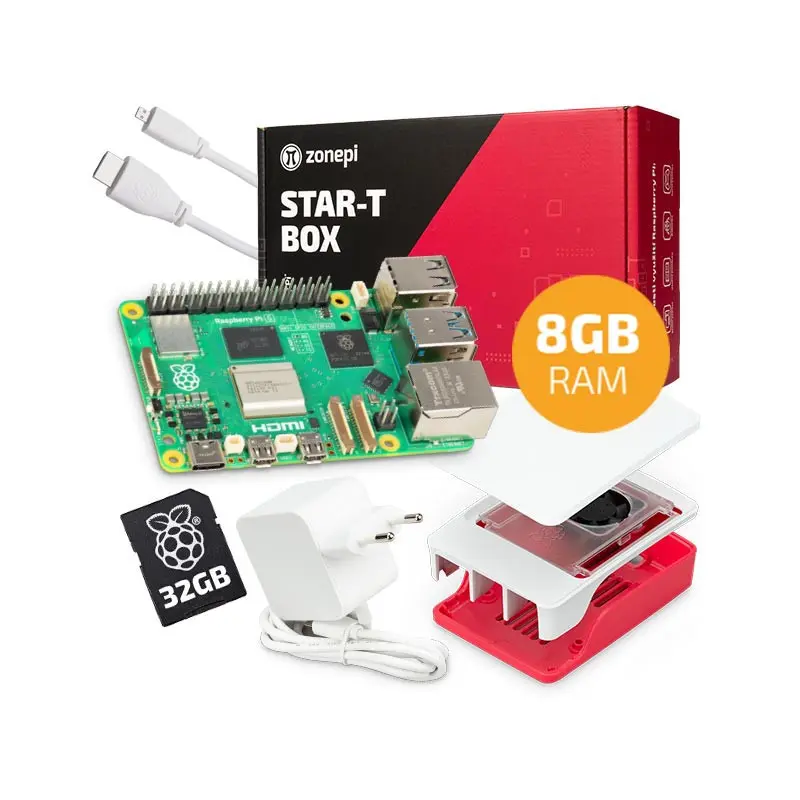
\includegraphics[scale=0.3]{./images/rpi.png}
	\centering
	\caption{Balíček s Raspberry Pi 5 \\ Zdroj: https://rpishop.cz/startovaci-sady/6508-oficialni-sada-s-raspberry-pi-5-8gb-ram-krabicka-32gb-microsd-prislusenstvi.html}
\end{figure}

\subsection{Celkové porovnanie}

\begin{table}[h]
\centering
\begin{tabular}{|l|c|c|c|}
\hline
\textbf{ } & \textbf{Moje riešenie} & \textbf{Komerčné riešenie} & \textbf{DIY riešenie} \\ \hline
\textbf{Cena bez zdielaných položiek (€)} & 365,78 & 689 & 135,86 \\ \hline
\textbf{Celková cena (€)} & 830,97 & 1154,19 & 601,05 \\ \hline
\end{tabular}
\caption{Porovnanie cien pre rôzne riešenia}
\end{table}


\section{Záver}
Z cenových porvnani vyplýva že náš systém NAS vychádza lacnejšie ako komerčné riešenie. Taktiež je oveľa viac konfigurovateľný a môžeme si ho prispôsobiť podľa našich potrieb. Avšak pre náročnejších ľudí, ktorý sa radi hrajú s rôznymi technológiami by bolo DIY riešenie s pomocou Raspberry Pi prípadne špecializovaného hardvéru za podobnú cenu lepšou voľbou. Nemá síce obrovský výkon ale ide zaujímavý projekt na ktorom sa dá veľa naučiť a zároveň ako obyčajné úložisko dát bez multimediálneho servera by bolo dostačujúce.

\pagebreak

\bibliography{literatura}
\bibliographystyle{unsrtnat}
\end{document}